\documentclass[10pt]{article}
\usepackage[utf8]{inputenc}
\usepackage[spanish]{babel}
\usepackage[usenames,dvipsnames,svgnames,table]{xcolor}
\usepackage{multirow}
\usepackage{diagbox}
\usepackage{booktabs}
\usepackage{anysize} 
\usepackage{hyperref}
\usepackage{helvet}
\renewcommand\refname{Referencias}
\marginsize{2cm}{2cm}{2.0cm}{2cm}
\usepackage{enumitem}
\usepackage{setspace}
\usepackage{scrextend}
\addtokomafont{labelinglabel}{\sffamily}

%% Graphics
\usepackage{graphicx}
\usepackage{color}
\usepackage{gensymb}
\usepackage{multirow}
\usepackage{caption}
\usepackage{float}


\hypersetup{
	colorlinks=true,
	linkcolor=blue,
	filecolor=magenta,
	urlcolor=cyan,
	citecolor=blue
}





\begin{document}
	\title{Fundamentos de Bases de Datos \\
		Practica 4\\ Modelo Relacional
	} 
	\author{}
	\date{19 de Marzo del 2019}
	\maketitle
	
	
	\section{Modificaciones al diagrama E-R del caso de uso}
	\begin{figure}[H]
		\centering
		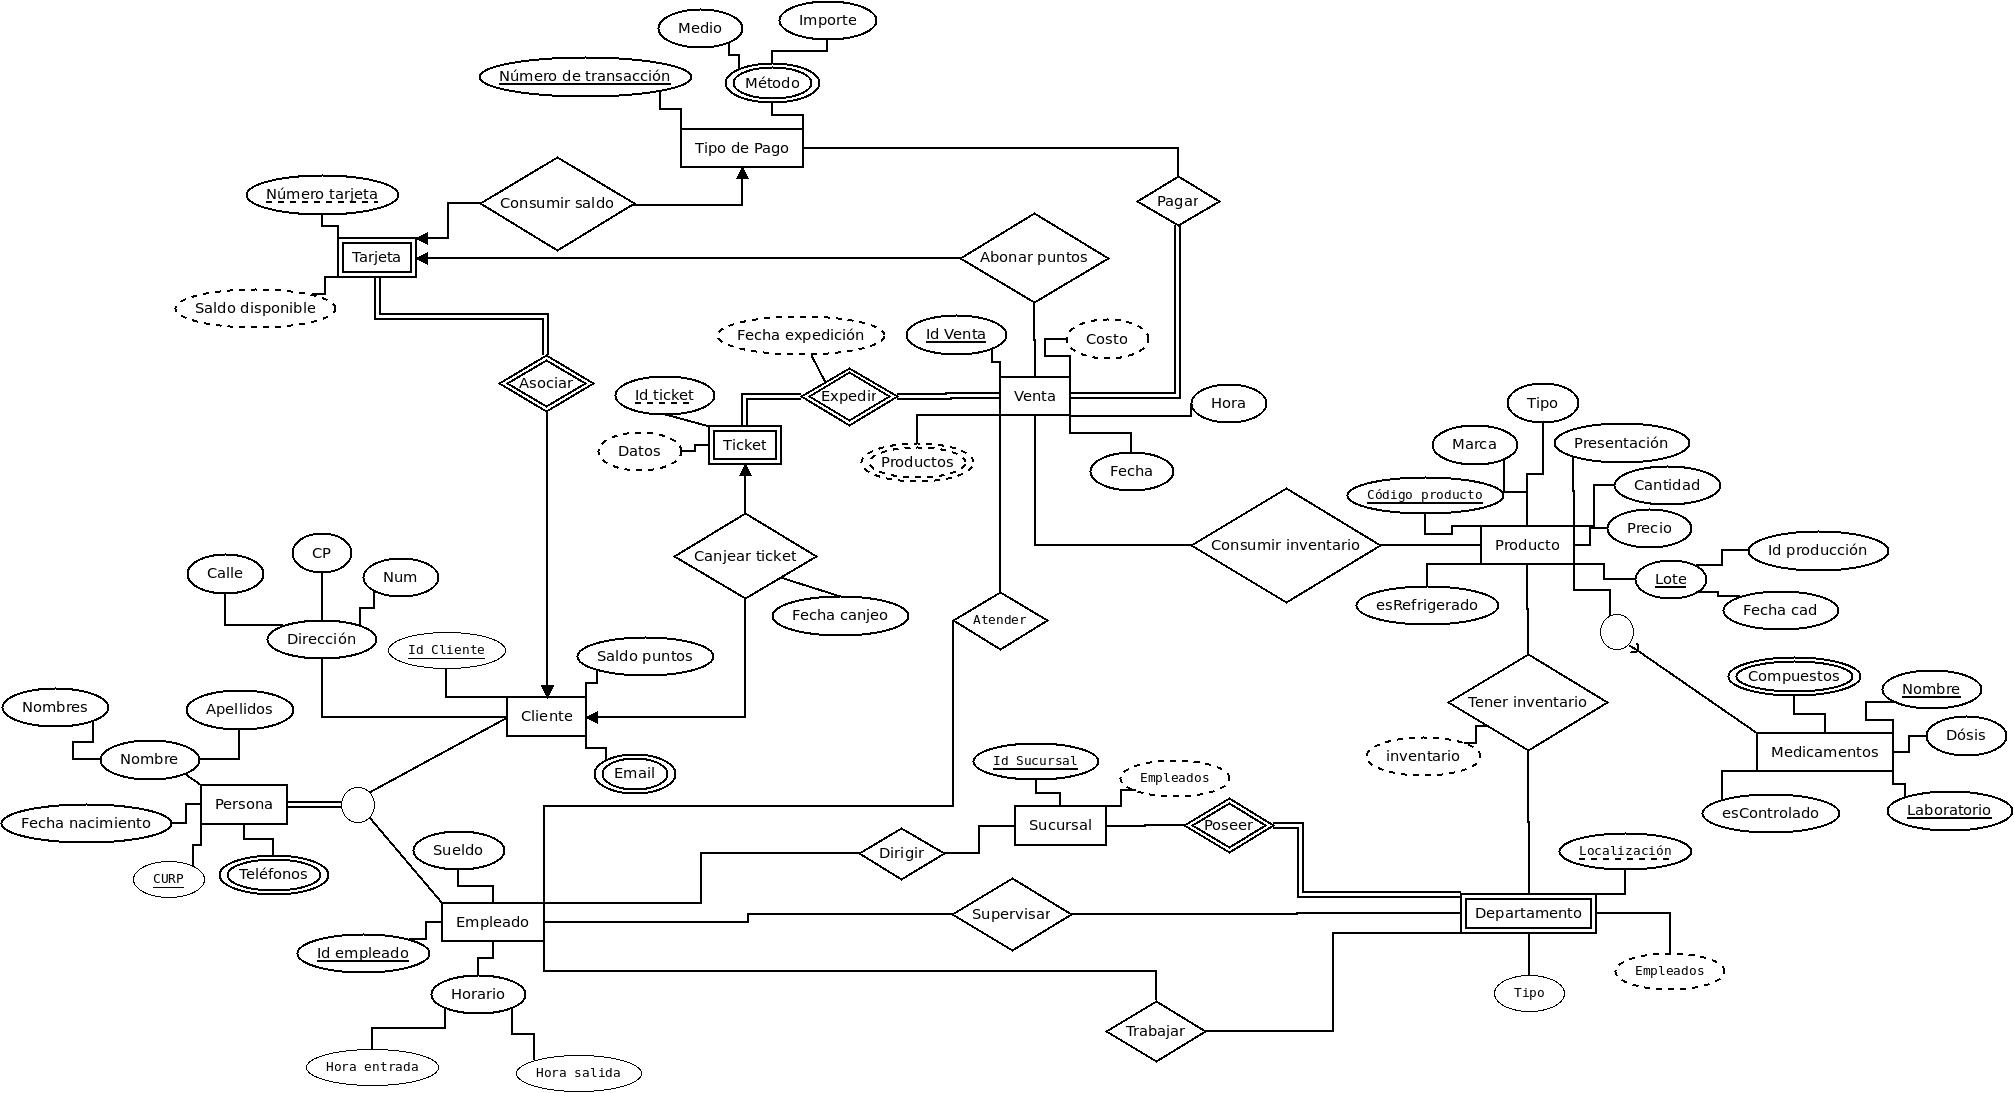
\includegraphics[width=1 \textwidth]{diagrama.jpeg}
		\caption{Diagrama E-R modificado para "\,El rey de los Abarrotes ".}
	\end{figure}

   \subsection{Correcciones}
   
   \begin{itemize}
   	\item Se hizo la corrección de ticket a entidad débil ya que desde un principio se había decido que sería así pero en el diagrama original se omitió por error.
   	
   	\item En el atributo Nombre de la entidad persona se agregó que este es un atributo compuesto por Nombre, Apellido Paterno y Apellido Materno. Además a  la entidad Persona se le modificó su llave primaria por CURP como llave primaria. 
   	
   	\item El atributo Dirección en la entidad Cliente se especifico que este es un atributo compuesto por Calle, Numero Ext, Número Int y CP. Además se le agregó a la entidad cliente su llave primaria Id Cliente que en el diagrama de la practica anterior por errores de diseño se omitio.
   	
   	\item Se quito las entidades Encargado y Gerente que heredaban de la entidad Empleado porque eran innecesarias para el modelo.
   	
   	\item También se decidio quitar las entidades que heredaban de Departamento y ponerlas como un atributo (Tipo) porque se iban a generar tablas sin mucha información.
   	
   	\item En la entidad Medicamento se agrega su llave primaria compuesta por Nombre y Laboratorio.  
   \end{itemize}
   
   
   
   

	\section{Modelo Relacional del caso de uso}
	
	
	
	\begin{figure}[H]
		\centering
		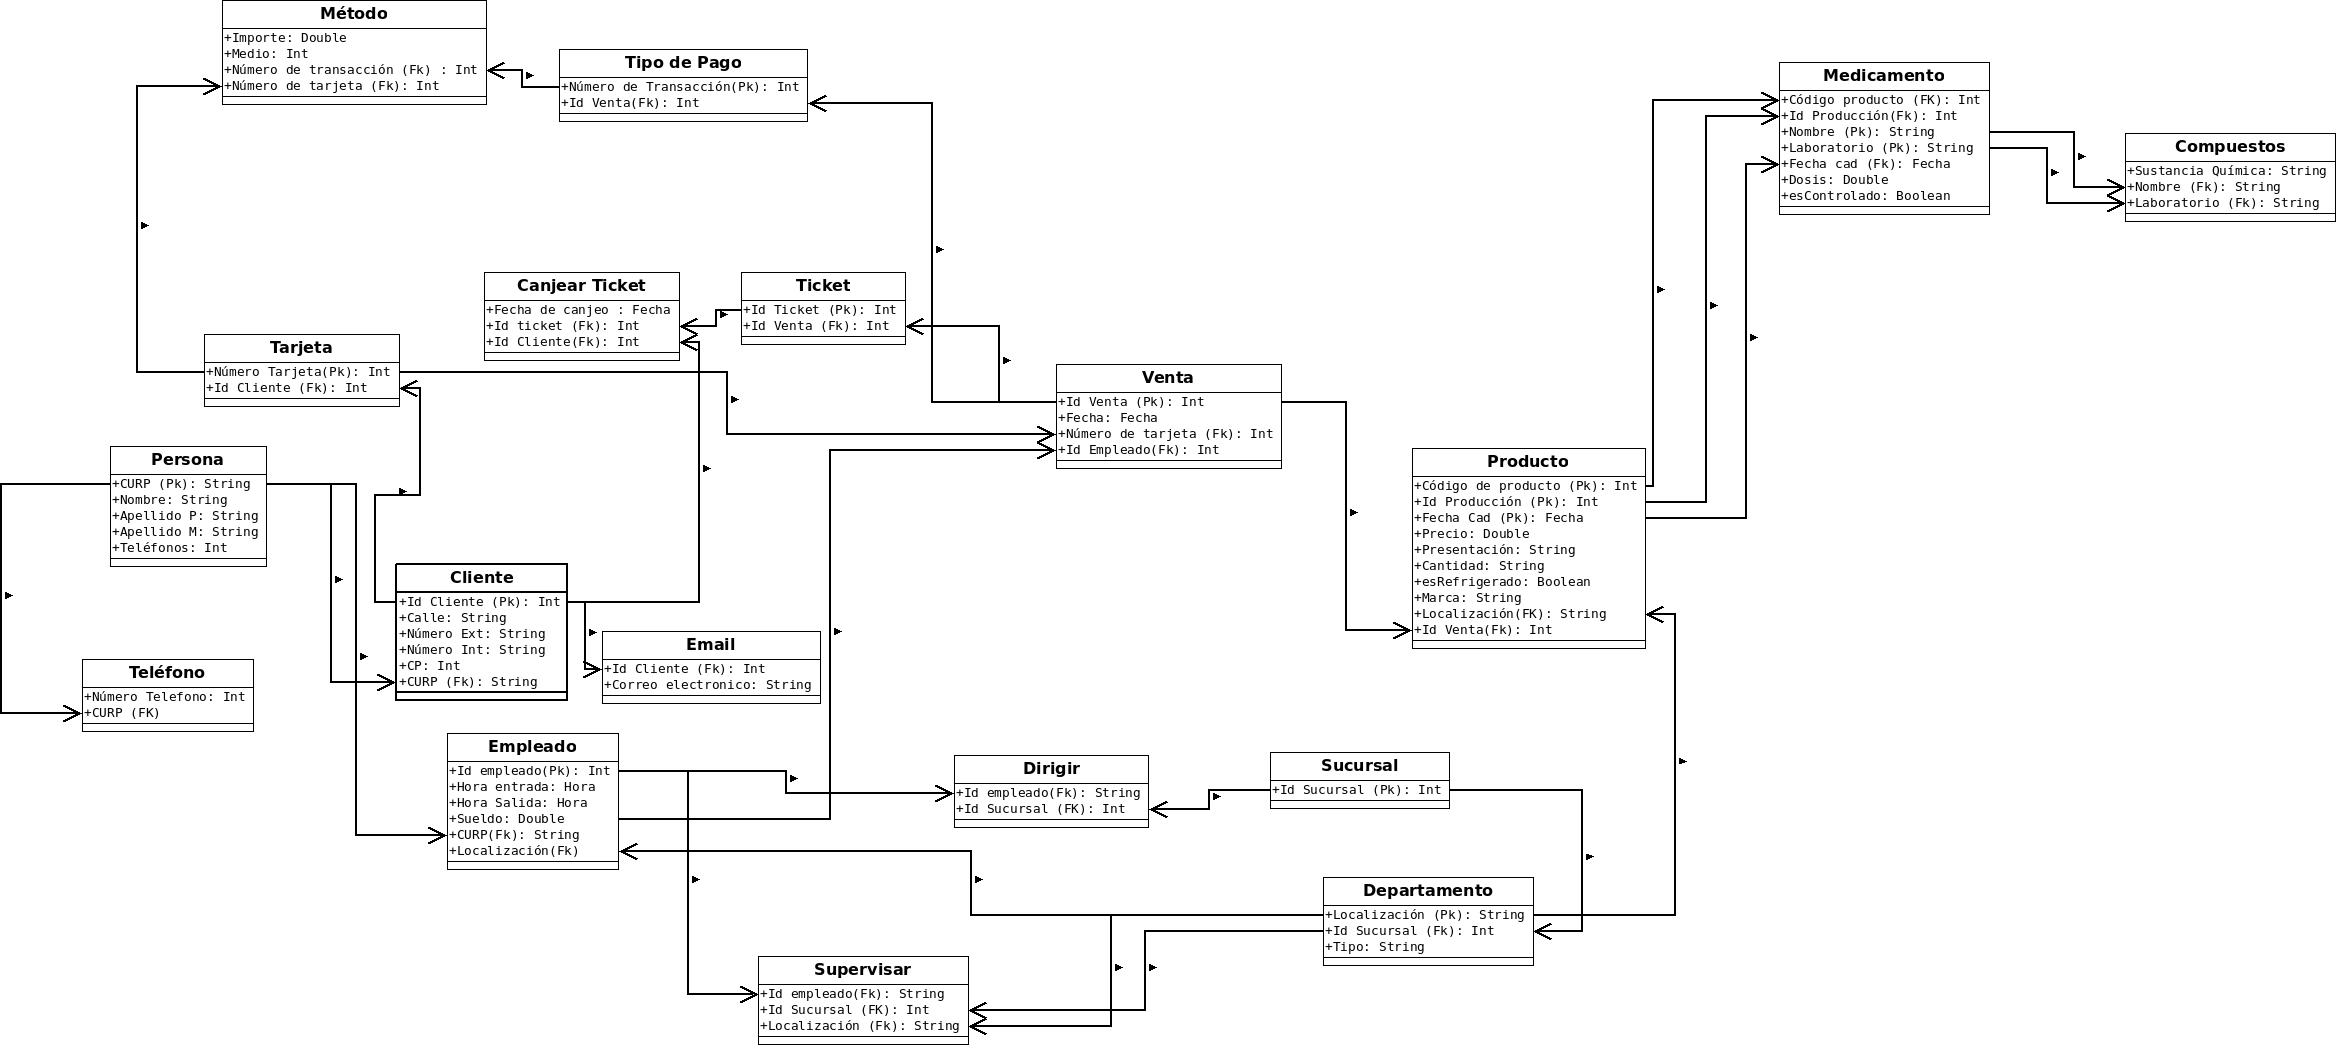
\includegraphics[width=1 \textwidth]{modeloRelacional.jpeg}
		\caption{Modelo Relacional para "\,El rey de los Abarrotes ".}
	\end{figure}
	

    
    \subsection{Relaciones}
    
    
    
    	
    	\begin{description}[leftmargin=9em,style=nextline]
    		\item[Trabajar] Pasa como llave foránea de Empleado.\\
    		
    		\item[Supervisar] Se crea una tabla que tiene como llaves foráneas los identificadores de Empleado y de Departamento donde la llave de departamento es una llave compuesta por Localización y el identificador de Sucursal. \\
    		
    		\item[Dirigir] Se convierte en una tabla que tiene como llaves foráneas: el identificador de empleado y el identificador de Sucursal . \\
    		
    		\item[Pagar] Pasa como llave foránea a Tipo de Pago.\\
    		
    		\item[Abonar puntos] Pasa como llave foránea a Venta. Esta llave puede ser nula
    		en el caso en que no se abonen puntos.\\
    		
    		\item[Expedir] Pasa como llave foránea a Ticket.\\
    		
    		\item[Atender] Pase como llave foránea a Venta.\\
    		
    		\item[Canjear ticket] Se convierte en una tabla que contiene el identificador de Empleado, el identificador de Ticket y la fecha de canjeo donde la fecha de canjeo debe ser menor a cinco días.\\
    		
    		\item[Consumir saldo] Originalmente esta relación iba a pasar como llave foránea a tipo de pago pero el atributo Metodo en tipo de pago genera una tabla al ser mutivaluado y se consideró mas adecuado que la relación fuese entre tarjeta y metodo, pasando como llave foránea en Método, esta llave puede ser nula en el caso donde no se pague con la tarjeta de puntos.\\
    		
    		\item[Tener inventario] Pasa como llave foránea a Producto. \\
    		
    		\item[Consumir inventario] Pasa como llave foránea a Producto. Esta llave puede ser nula lo que indicaría que el producto no se ha vendido. \\
    		
    		\item[Asociar] Pasa como llave foránea a Tarjeta. \\
    		
    		\item[Poseer] Pasa como llave foránea a Departamento. \\
    		
    	\end{description}
   

	
	

	
	
	
	
	\section{Bitácora}
	
	\begin{labeling}{alligator}
		\item [15/03] Inicio de proyecto.
            
            Durante esta reunión empezamos a traducir el diagrama E-R que se hizo en la practica pasada al modelo relacional. Se comenzó la traducción de las entidades a tablas. En el proceso se decidió hacer algunas modificaciones y correcciones al diagrama E-R.            
		\item [19/03] Sesión de laboratorio
		
		    Terminamos la traducción, complementando con la traducción de las relaciones a tablas, viendo que relaciones generaban tablas y cuales se añadia a una tabla existente como llave foránea.
		
            . 
    
		
       
        
	
		
	\end{labeling}
	
	
	
\end{document}
